\documentclass[runningheads]{llncs}

\usepackage{booktabs}
\usepackage{xspace}
\usepackage{hyperref}
\usepackage{graphicx}
\usepackage{comment}
\usepackage{caption}
\usepackage{subcaption}
\usepackage{float}
\usepackage{lipsum}
\usepackage{amsmath}
\usepackage{soul}
\usepackage{xcolor}
\usepackage{mathtools}


\newcommand{\fillcaption}[1]{Fig. \arabic{figure}: #1 } 

\newcommand{\todo}[1]{\textcolor{red}{\textbf{TODO: #1}}}
\newcommand{\red}[1]{\textcolor{red}{#1}}
\newcommand{\blue}[1]{\textcolor{blue}{#1}}
\newcommand{\hide}[1]{}

\makeatletter
\renewcommand{\fps@figure}{!ht}
\renewcommand{\fps@table}{!ht}
\makeatother

\newenvironment{colorpar}[1]{%
    \leavevmode\color{#1}\ignorespaces%
}{%
}%


%% Some important configurations here %%
\graphicspath{{../images/}, {../plots/experiment_}, {../plots/}}

\DeclarePairedDelimiter\ceil{\lceil}{\rceil}
\DeclarePairedDelimiter\floor{\lfloor}{\rfloor}

\newcommand{\poa}{proof-of-authority\xspace}
\newcommand{\Poa}{Proof-of-authority\xspace}
\newcommand{\pow}{proof-of-work\xspace}
\newcommand{\Pow}{Proof-of-work\xspace}
\newcommand{\rpi}{Raspberry Pi Zero~W\xspace}
\newcommand{\rab}{range-and-bearing\xspace}

\hyphenation{block-chain}
\hyphenation{block-chains}

%% Title and authors %%
% \title{Blockchain-based coordination of a foraging robot swarm} \titlerunning{Blockchain-based coordination of a foraging robot swarm}

%\title{Using blockchain smart contracts in real-time coordination of a foraging robot swarm} \titlerunning{Blockchain-based coordination of a foraging robot swarm}

\title{Real-time Coordination of a Foraging Robot Swarm using Blockchain Smart Contracts} \titlerunning{Blockchain-based coordination of robot swarms}


\author{Alexandre Pacheco\orcidID{0000-0001-5933-3553} \and Volker
  Strobel\orcidID{0000-0003-2974-9827} \and Andreagiovanni Reina\orcidID{0000-0003-4745-992X} \and Marco
  Dorigo\orcidID{0000-0002-3971-0507}} \authorrunning{A. Pacheco et
  al.}  
  \institute{IRIDIA, Universit\'e Libre de Bruxelles, Brussels, Belgium
  \email{alexandre.melo.pacheco@ulb.ac.be}}

	\index{Pacheco, Alexandre}
	\index{Strobel, Volker}
	\index{Reina, Andreagiovanni}
	\index{Dorigo, Marco}

\date{\today}

\begin{document}
\maketitle

% Some quotes and outtakes
%Cooperative foraging is most beneficial when food resources are unpredictable or scarce, as cooperative groups are likely to locate and exploit resources with greater efficiency than individuals (Wilson 2000).

 %Verified information is valuable in applications where the correctness of information is paramount. Before being definitely included in a blockchain database, information undergoes a verification process which is designed as Byzantine fault-tolerant. The messages exchanged in blockchain networks are also non-repudiable, which ensures that agents are accountable for the information they provide to their peers. These properties are crucial to ensure that information aggregated by a large network of swarm agents is secure. On the downside, blockchain consensus introduces latency which we hypothesize may limit its use for high-level, or safety-critical, control rules, while lower level routines continue to be executed locally by each robot. In this fashion, blockchain feedback can be interpreted as a decentralized coordinator whose function is to extend the swarm's ability to self-coordinate and thus improve the collective performance.
 
 %In swarm robotics research, the communication abilities of robots are often constrained in order to achieve distributed and leaderless systems. On one hand, these constraints guarantee that robot swarms are robust to singular points-of-failure; but on the other hand they also restrict the control ability of the swarm and often lead to swarms which perform well on certain environments, but fail to adapt (change algorithms or tasks) when the environmental conditions change \cite{hoff_distributed_2013}. To avoid centralized supervision, researchers have proposed hybrid swarms \cite{mns} which address task allocation by allocating some decision-making power to coordinating robots.

 %This is especially relevant when the information is requested for safety-critical applications; or when it is utilized by the robots control algorithms, since false information could potentially lead to unstable feedback loops.
 %To implement high-level decision rules which all robots agree with and enforce in a decentralized manner.
 
 %In literature, decision-making and coordination in robot swarms typically emerges from local and simple interactions between robots. While this design choice promotes scalability, it also generates what is known as the micro-macro link  is no unified framework to relate individual behaviors and swarm behaviors. %oftentimes, not achievable as there is a lack of means for robots to agree on the state of the environment, and furthermore, on a single action policy.
 
\section{Introduction}
\label{sec:introduction}

The application of blockchain technology to robotic systems is a fast growing research topic. Particularly, in swarm robotics, the most noteworthy advancement was the introduction of a blockchain in order to achieve secure consensus in the presence of Byzantine agents \cite{StrCasDor2020_frontiers,pacheco_ants_2020}. Blockchain-secured robot swarms could be deployed in situations where security against unauthorized agents is paramount; or in open-swarm scenarios, in which robots are deployed by different, untrusting parties.
 
The proposition of a \emph{decentralized} and \emph{secure} database has the potential to introduce a paradigm shift in the field of swarm robotics. However, further research is required to understand the extent of the disruption, as well as its drawbacks. 

Ethereum~\cite{buterin_2014_ethereum}, launched in 2015, extended the original application of blockchains from financial ledgers to decentralized computing platforms. While early blockchains, such as Bitcoin~\cite{bitcoin_online}, allow participants to agree on the execution of financial transactions, participants in the Ethereum network can also agree on the execution of computers programs known as \emph{smart contracts}. 
 
In this work, we argue and validate the claim that smart contracts can be very valuable when applied to the real-time coordination of robot swarms: a smart contract is control code that is executed in a decentralized manner by the swarm, i.e., each robot executes the code independently and the swarm comes to an agreement on the the output of the control code. On a micro perspective, the robots maintain the local behaviours and interactions typical of swarm robotics literature, while on a macro perspective, the blockchain provides an extension to the swarms' ability to coordinate and self-organize. 

%However, this scheme for decentralized programming introduces a consensus delay which could limit its applications to high-level (and safety-critical) control. There is yet no research which explores the viability of the blockchain as an element of the robots' control and decision making process. 

To validate this claim, we deploy a blockchain to act as a decentralized coordinator during a swarm foraging task. Robots broadcast transactions that contain data they obtained from scouting the environment for resources. The blockchain protocol guarantees that these transactions are executed orderly and conflict-free, and that all robots reach a agree on the most recent state of the resource database. Furthermore, the smart contract distributes the available robots (recruits) to the various resources (prioritizing resources with better quality), while limiting the number of foragers per resource in order to reduce physical collisions. These simple rules are shown to increase the collection rate and energy efficiency during the foraging task. 
The consensus protocol that is used is \poa~\cite{poa_online}, which we have shown in previous research \cite{StrCasDor2020_frontiers,pacheco_ants_2020} to be suitable for robot swarms since it requires low power and is robust to networking partitioning or temporary unavailability of consensus agents (up to 50\% of all authorized agents).

In section~\ref{sec:related-work} we look at the related work on the topics of blockchain applied to robot swarms and cooperation in foraging robot swarms. In section~\ref{sec:methods} we introduce the foraging task, the environment, and other methods relevant for the implementation of the experiments: the simulations software, the blockchain protocol, the robot's model and controllers. In section~\ref{sec:results-and-discussion} we show and discuss the experimental results. In section~\ref{sec:conclusion} we deliver the conclusions of this study and provide guidelines for future research.


\section{Related Work}
\label{sec:related-work}

\subsection{Cooperation in foraging robot swarms}
\label{sec:rw-foraging}
Foraging is one of the most studied behaviours in swarm robotics, due to its wide range of application scenarios: search and rescue, agriculture, mining, waste cleaning and planetary exploration, for instance. It can be described as the combination of two sub-tasks: 1)~searching the environment for objects; 2)~and performing an action on those objects (e.g. transportation, consumption or destruction). 
In this work we focus on central place foraging \cite{houston_general_1985}, where agents are tasked with finding and transporting objects back to a target location (the nest). 

Inspired by the foraging behaviour of ants, which deposit pheromones along paths leading to objects \cite{deneubourg_ants_1990}, robot swarm algorithms are most often based on indirect communications (stigmergy). Researchers have attempted to mimic the ants behaviour using chemicals~\cite{salman_phormica_2020}; augmented reality pheromones~\cite{font_llenas_pheromones_2018}; or virtual pheromones~\cite{campo_artificial_2010,hoff_distributed_2013} which are advertised locally by robots which are assigned the role of pheromone beacons. The main advantage of these methods is scalability and robustness, however, they have been shown to converge to sub-optimal solutions~\cite{missing}, particularly when malicious agents are present~\cite{pincy_hacking_2022}.

For these reasons, some researchers have adopted forms of direct communication. The scout-recruit model is inspired by the recruitment dances that honeybees perform to signal the location of objects to peers \cite{seeley_bees_1983,biesmeijer_exploration_2001}.

% SHORTER ALTERNATIVE TO TWO PARAGRAPHS ABOVE
% Inspired by the foraging behaviour of insects, robot swarm algorithms are most often based on indirect communications (such as stigmergy~/cite{deneubourg_ants_1990, salman_phormica_2020, font_llenas_pheromones_2018, pincy_hacking_2022}); or direct communications (such as the recruitment dance of honeybees~\cite{biesmeijer_exploration_2001}). In this work, we focus on the scout-recruit model~\cite{seeley_bees_1983}, as a form of coordination through explicit communications.

 Pitanokova et al. \cite{pitonakova_understanding_2014,pitonakova_icr_2018} compare swarms where robots recruit others at the nest, versus swarms of individualist foragers. They show that when resources are scarce or difficult to find, nest-site recruitment can be helpful to maximize the total resources collected. Conversely, in resource-abundant environments it may be more advantageous to forage individually, and thus prevent \emph{physical interference} (when robots foraging for the same resources collide) and \emph{informational interference} (when the information exchanged is outdated or incorrect). Similar observations have also been noted in nature \cite{wilson_sociobiology_2000}. Despite this insight, no coordination strategy nor methodology to enable the validation of the information are proposed in order to limit or reduce interferences.

\subsection{Applications of blockchain to swarm robotics}
\label{sec:blockchain-applications}

The concept of blockchain-based robot swarms was introduced in 2016~\cite{ferrer_blockchain_2016}. The author proposes that the integration of a blockchain could help address issues such as data integrity, consensus agreement, and secure communication in decentralized robot networks. In~\cite{StrCasDor2018_aamas,StrCasDor2020_frontiers}, the authors present a proof-of-concept (in simulation) showing how blockchain-based smart contracts can be exploited to neutralize the negative effect of Byzantine robots in a consensus problem. In~\cite{PacStrDor2020:ants} the authors present the first implementation of a blockchain in a swarm of real robots using Ethereum's~\cite{buterin_2014_ethereum} \poa consensus, which is shown to be suitable to robot swarms given that it is energy efficient, scalable and robust to a reasonable degree of network partitioning.

 Although these studies showcase the promise of smart contracts to achieve generic swarm-wide agreements, it is not yet clear if the network consensus delay is too large to allow a wider range of applications, particularly, real-time control. Some researchers avoid the question altogether by presenting some control architectures in which the blockchain is hosted outside of the swarms' network~\cite{outsidehosting}. This scheme is akin to using an external control element (albeit, a distributed one in this case), and does not grant the autonomy and fault-tolerance properties warranted in a robot swarm. In this work, we present and study a decentralized and autonomous blockchain-based robot swarm that exploits smart contracts for real-time coordination.

\section{Methods}
\label{sec:methods}

\subsection{Description of the task} 
The goal of the swarm is to retrieve resources from the environment and deposit them at the nest site. Each experiment has a duration of $15$~minutes. When a resource is deposited at the nest, the \emph{total reward collected} is incremented according to the quality of the resource (see below). The \emph{scouting efficiency} is calculated offline as the ratio between the \emph{total reward collected} and the \emph{total distance travelled} by the robots while they are exploring the environment for resources. 

\subsection{Description of the environment}
\label{subsec:env}

The environment consists of a square arena with a side length equal to $2.89$~meters in the experiments with $25$~robots ($3$~robots per square meter). The nest is a circle at the center of the arena with a diameter of $0.98$~meters (Figures~\ref{fig:abundant}--\ref{fig:litter}). Robots deposit resources on the external annulus of the nest, while the interior is reserved for idling. The nest additionally has a beacon which broadcasts an homing signal, which allows robots to securely navigate back to the nest from any location. The remainder of the arena is covered by a variety of circles which represent resource \emph{patches}.

Resource \emph{patches} are distributed in an annulus around the center of the arena, where the minimum distance is $0.83$~meters and the maximum distance corresponds to half the arena size. This is done to prevent patches from spawning too close to the nest, or too far, in the corners of the square arena. Each patch is a circular area that contains multiple \emph{resources} that the robots can scout and forage. After all resources in a patch are collected, a new identical patch is generated elsewhere.

The \emph{resources} can have different qualities, and thus, different rewards when foraged by the robots: red (reward $2$), green (reward $4$), blue (reward $6$) and yellow (reward $8$). 
The distribution of resources in the arena can be tuned by parameters in a configuration file. We consider $3$~different distributions:

\vspace{-4mm}
\subsubsection{Scattered distribution} 
In the scattered distribution $3$\% of the environment floor area is covered with uniformly distributed patches. Each patch has a diameter of 12~cm and contains $10$~resources. 70\% of the patches are red, while there is 10\% of each green, blue and yellow.

\vspace{-4mm}
\subsubsection{Concentrated distribution}
The concentrated distribution has the same environment floor area covered as the scattered distribution. However, each patch has a larger size of 30~cm and contains $15$~red or blue resource. 

\vspace{-4mm}
\subsubsection{Hotspot distribution} 
In the hotspot distribution, again $5$\% of the environment floor area is covered with patches. however they are all concentrated on the first quadrant of the arena. Each patch has a diameter of 12~cm and contains $10$~red resources. 


\begin{figure}
     \centering
     \begin{subfigure}[b]{0.49\textwidth}
         \centering
         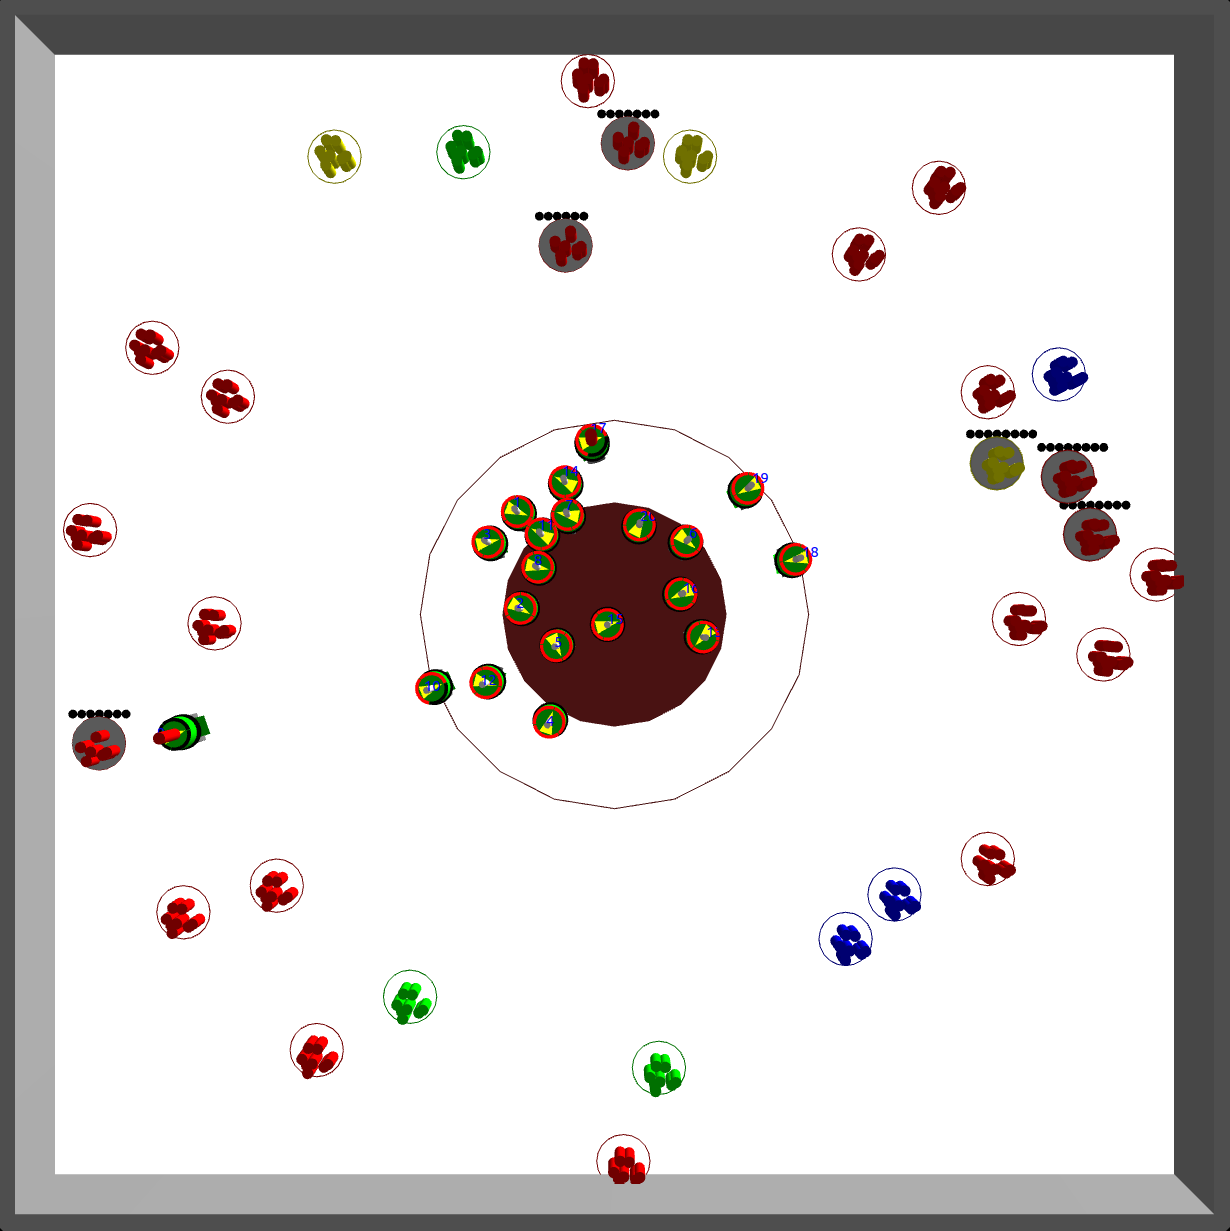
\includegraphics[width=\textwidth]{abundant.png}
         \caption{Scattered distribution}
         \label{fig:scattered}
     \end{subfigure}
     \hfill
     \begin{subfigure}[b]{0.49\textwidth}
         \centering
         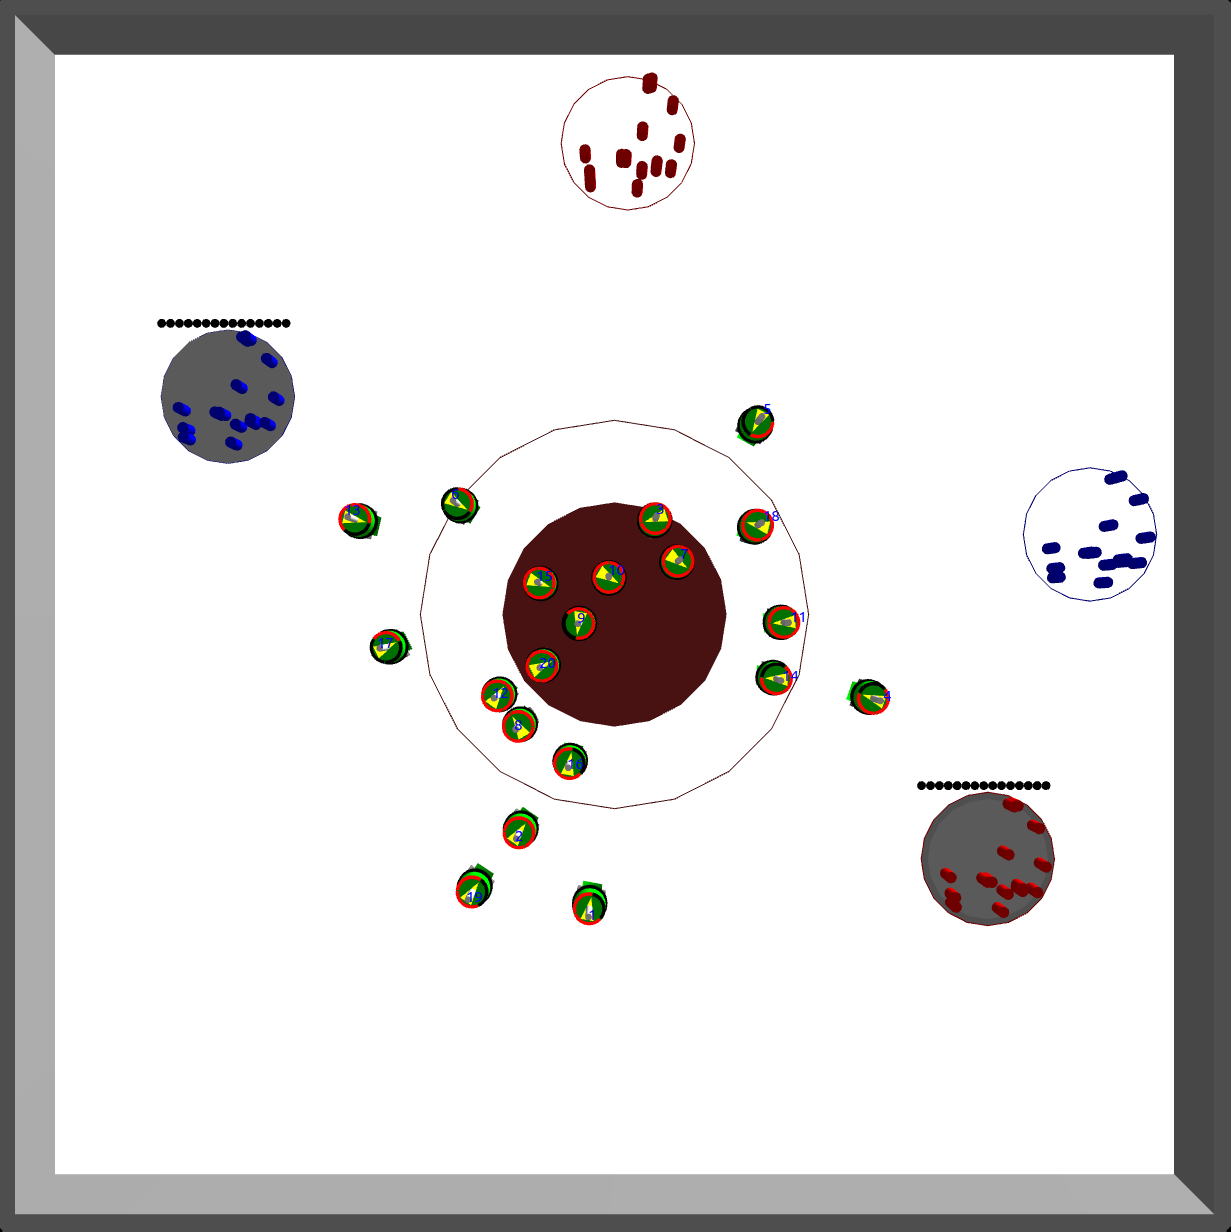
\includegraphics[width=\textwidth]{scarce.png}
         \caption{Concentrated distribution}
         \label{fig:concentrated}
     \end{subfigure}
     \hfill
        \begin{subfigure}[b]{0.49\textwidth}
         \centering
         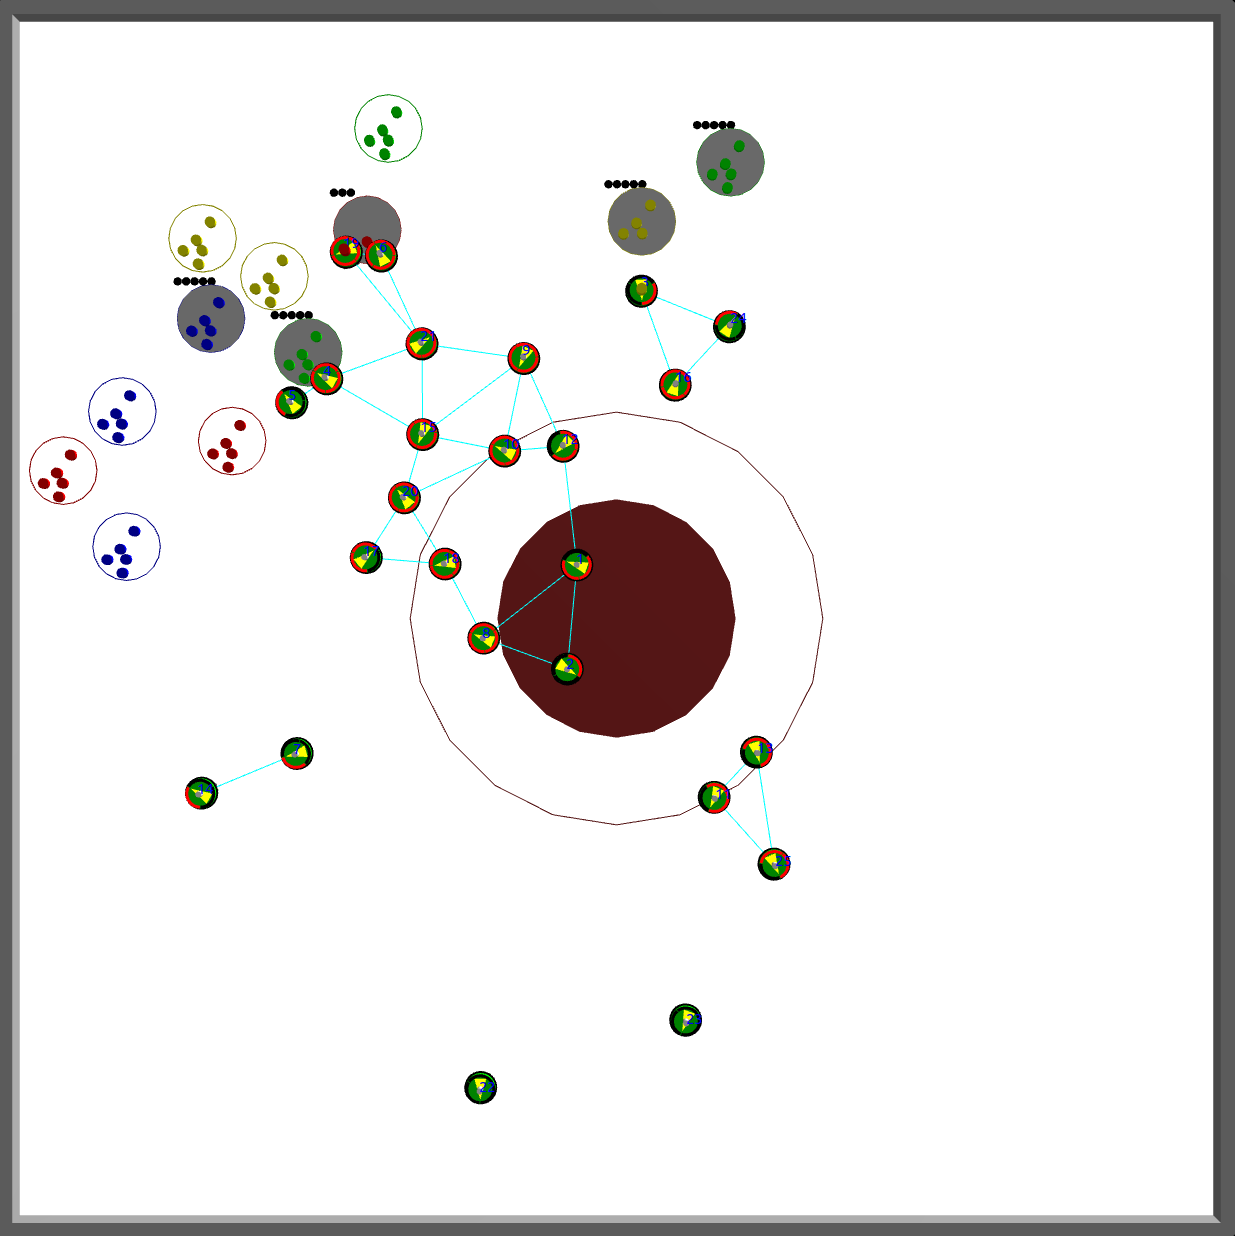
\includegraphics[width=\textwidth]{hotspot.png}
         \caption{Hotspot distribution}
         \label{fig:hotspot}
    \end{subfigure}
    \begin{subfigure}[t]{0.49\textwidth}
        \centering
        \vspace{-35mm}
        \fillcaption{Figure legend here}
    \end{subfigure}

\end{figure}


\subsection{Description of the simulations setup}

The simulation setup comprises the swarm robotics simulation software ARGoS~\cite{pinciroli_2012_si_argos}; the blockchain software Ethereum~\cite{buterin_2014_ethereum}; and the virtualization software Docker~\cite{merkel_2014_docker}. Docker is used to create virtual containers which run the nodes of a custom Ethereum network and host their client interfaces (\texttt{geth}) via TCP servers. Each ARGoS robot controller is associated with an Ethereum node, and can interact with that respective client using the TCP connection.
In this way, the ARGoS robot controllers only interact with the client-side API of Ethereum (for example, to send transactions, make database queries or add/remove peers), while the execution of the Ethereum core (blockchain maintenance) is performed by the Docker containers in the background.
 
 To unify these components into a single framework, we use Python wrappers for both ARGoS~\cite{ken_argos_python}, and \texttt{geth}~\cite{web3py_2022}. This allows the robot control routines and interactions with the blockchain client to be fully written in Python. Data analysis and plotting is also performed using Python. A full description of the simulations setup was published as a technical report \cite{PacStrDor2020_techreport}, and is available on Github~\cite{teksander_argos_geth_github}.

\subsection{Description of the blockchain}
 Ethereum~\cite{buterin_2014_ethereum}, launched in 2015, extended the original application of blockchains from decentralized financial ledgers to decentralized computing platforms. While financial ledger blockchains, such as Bitcoin~\cite{bitcoin_online}, allow participants to agree on the execution of financial transactions, participants in the Ethereum network can also agree on the execution of computers programs known as \emph{smart contracts}. Due to their decentralized nature, blockchains require a \emph{consensus protocol} in order to solve conflicts and agree on the same version of the blockchain. %In this section, we explain the concepts of consensus protocol and smart contract, and describe how they are used in our experiments.

\subsubsection{Consensus protocol}
\label{sec:consensus-protocol}
\Pow~\cite{bitcoin_online}---the original and most commonly used blockchain consensus protocol---requires the expenditure of computational resources in order to establish which blocks of information are added to the blockchain. For this reason, it is often regarded as counter-indicated for swarm robotics applications, which typically consider robots with limited capabilities and resources \cite{dorigo_swarm_2008}.
In our research, we have introduced \poa~\cite{poa_online} as an alternative to \pow. \Poa keeps a core of authorized and accountable nodes which share the role of producing (sealing) new blocks. In this protocol, anyone can create a block and propose it, but in order for a new block to be valid:
\begin{itemize}
\item the difference between the timestamp of the new block must be at least $t=B_p$ seconds ($t=B_p$ is called the \emph{block period});
\item the proposed block must be correctly signed by an authorized sealer using its public key;
\item a sealer can only sign one block every $\floor{\frac{N}{2}} + 1$ blocks.
\end{itemize}
Every node in the network checks if the proposed blocks meet these conditions. If they are met, the node appends that block to its local copy of the blockchain. The consensus protocol establishes that the current version of the blockchain is the one which has the highest \emph{cumulative difficulty}. Blocks which are sealed \emph{in-turn} (i.e., that are sealed by an appointed preferred sealer for that block), contribute with a difficulty of 2; while other blocks contribute with 1.

Blockchain forks can occur temporarily, for instance, when preferred sealers are unavailable in a partitioned network or when there is excessive communication delay. To increase the confidence that information is permanently added to the blockchain, nodes can wait for the cumulative difficulty to increase. Unreliable sealers (faulty robots for instance) can be voted out by majority vote, and new sealers may also be voted in. As such \poa is suitable for dynamic swarms, since robots can join and leave the swarm at anytime during the execution of the collective task.

\subsubsection{Blockchain smart contract}
\label{sec:smart-contract}

A blockchain smart contract is a computer program that is stored on the blockchain, and that encapsulates code (its functions) and data (its state). Network participants can execute its functions by sending transactions to the smart contract address, which in turn will change its state. It is the role of the blockchain system to agree on the irrefutable execution of these transactions in a decentralized and trustless manner.

The smart contract used in this experiment allows robots:~1) to store information regarding discovered resource locations;~2) to enlist themselves as recruits in order to forage at a certain location; and~3) to query information about the known resource locations. In this fashion, the smart contract can be interpreted as a decentralized coordinator whose function is to extend the swarm's ability to self-organize, and thus improve the collective performance. The smart contract coordinator additionally regulates swarm behaviour by establishing a limit on the number of foragers allowed per patch, and by aggregating the information provided by the robots in a conflict-free database, thus reducing both physical and informational interference.

Our smart contract offers three functions that the robots can interact with:
\begin{itemize}
	\item[$\bullet$] \texttt{scout(string resource\_json)} - the input is a formatted string containing position, radius, quality and quantity of the resource. If the position is unique (within an error margin) a new resource is added to a list, otherwise the information about a current resource at at location is updated;
	\item[$\bullet$] \texttt{recruit()} - assigns the highest quality available resource to the caller (the caller becomes a recruit). If that resource currently has the maximum number of recruits assigned, the next best quality resource is assigned;
	\item[$\bullet$] \texttt{get\_resources() return list} - returns a list with all resources and relevant information about them.
\end{itemize}

\subsection{Description of the robot model (Pi-puck)}
The agent used in the simulations is a model of the Pi-puck robot~\cite{millard_2017_iros_pipuck}. In previous research, we showed that 1)~the Pi-puck robots are capable of executing the blockchain software~\cite{pacheco_ants_2020}; and 2)~that the simulation setup we use provides an accurate approximation of the real swarm behavior~\cite{StrCasDor2018:aamas}. 

The Pi-puck model includes sensors and actuators required for this experiment: infrared sensors (used for obstacle avoidance); a \rab board (used for local peer discovery); a ground sensor (sensing of colored resource sites); and two motors (for locomotion). The real robot has no gripper or actuator to manipulate foraged resources, as such resource collection and depositing is performed virtually.
 
\subsection{Description of the robot controller}
The robots are controlled through a \emph{finite-state machine} composed of 6 states. The robot starts in state\texttt{Idle.IDLE}, and at each simulation step it performs a routine according to its current state and verifies the transition conditions. Additionally, the \emph{blockchain peer discovery} is performed at the beginning of every simulation step, regardless of the robot state.

\subsubsection{Finite state machine}
\label{sec:finite-state-machine}
\begin{itemize}
\item \texttt{Idle.IDLE} - The robot waits for a fixed amount of time ($30$~seconds) and then transitions to \texttt{Scout.EXPLORE};
\item \texttt{Idle.PLAN} - The robot queries \texttt{get\_resources() return list}. If the robot is enlisted as a recruit, it transitions to \texttt{Recruit.FORAGE}. Otherwise, the robot transitions to \texttt{Recruit.TRANSACT};
\item \texttt{Scout.EXPLORE} - The robot performs a random-walk for an amount of time taken from an normal distribution $\mathcal{N}(\mu=26,\sigma=5)$ and records the scouted resources locally. Afterwards, it transitions to \texttt{Scout.TRANSACT};
\item \texttt{Scout.TRANSACT} - The robot transacts \texttt{scout(string resource\_json)} for each scouted resource and deletes it from local storage. After the last transaction is successfully included in a block and confirmed (minimum 3 blocks), it transitions to \texttt{Idle.PLAN};
\item \texttt{Recruit.TRANSACT} - The robot transacts \texttt{recruit()} to be assigned a new resource for foraging. If the transaction is successfully included in a block and confirmed (minimum 3 blocks), it transitions to \texttt{Idle.PLAN}. Otherwise, there are no resources available and the robot transitions to \texttt{Idle.IDLE};
\item \texttt{Recruit.FORAGE} - The robot navigates from the nest towards the direction of the resource and searches the neighbourhood for $10$~seconds or until a resource is found a collected. Afterwards, the robot returns to the nest and transitions to \texttt{Scout.TRANSACT}.
\end{itemize}

\subsubsection{Blockchain peer discovery}
\label{sec:peer-discovery}
The robots use the \rab board to broadcast their IP address (up to $30$~cm). If this communication is reciprocated, each robot sends its enode via TCP. The enode is a unique identifier that the robots use to add and remove peers using \texttt{geth}. After the short-range signal is lost, each robot deletes the peer from local memory and from the list of blockchain peers. 

Our blockchain peering scheme serves two purposes: 1)~to ensure that communications are only local and thus mimic a real-world swarm deployment where network partitioning can occur; and 2)~to provide an additional layer of security which prevents external agents from participating in consensus, as the robots reject connections which are not accompanied by the short range greeting.

\section{Results and Discussion}
\label{sec:results-and-discussion}

In general, our goal is to show that by deploying a blockchain we can optimize the behaviour of the swarm by aggregating information from the robots in a conflict-free manner, and leveraging this information to coordinate the robots' actions, while maintaining the important properties of a robot swarm: \emph{decentralization}, \emph{adaptability} and \emph{scalability}.

The blockchain allows robots to agree on the state of the environment and on a shared coordination strategy, without the need for delegated supervisors (in contrast with centralized or hybrid control). Instead, the blockchain enables a decentralized and democratic swarm, in which all robots contribute homogeneously to the decision-making process. Such a system is robust to network partitioning, and can thus adapt to situations where a system that relies on information traveling to and from supervisors would fail (for example, in environments with limited or no communication infrastructure). 

The catch lies in the form of \emph{consensus latency}, i.e., the time it takes for messages to travel between robots and to be verified in this democratic process---and in \emph{data storage costs}, since each robot keeps a local copy of the blockchain database. These aspects raise scalability concerns in terms of communications and hardware requirements. In section~\ref{subsec:scalability} we discuss these concerns.

Cooperation is not always an advantage~\cite{pitonakova_icr_2018}. Sharing information can lead the swarm to over-exploit already known resources and miss out by not exploring for better resources. It also leads to higher physical interference (due to the increase in robot collisions) and informational interference (due to the broadcasting of incorrect/outdated information). The role of our smart contract coordinator is to optimize the foraging task (in terms of \emph{total reward collected} and \emph{energy efficiency}) by aggregating the latest known resource information from robot scouts, and allocating resources to robot recruits, thus minimizing the impact from both forms of interference. In section~\ref{subsec:performance} we show the performance results of a blockchain-coordinated robot swarm in comparison with an uncoordinated swarm, in environments with different resource distributions, and when the maximum number of recruits allowed by the smart contract increases.

%In results section A, we compare two robot swarms in which the individual robots perform the same control routine, but with one key difference: one swarm does not use a blockchain and thus the robots forage resources based on their own scouting and local data. In contrast, the robots in the second swarm do not keep any information locally. Instead, they transact to store the resource information on the blockchain and perform foraging based on the information that they have added to the blockchain. In this fashion, we seek to draw conclusions regarding the aforementioned scalability concerns of a blockchain-controlled approach to swarm coordination.

%In experiment B, we analyze the performance of a $20$~robot swarm performing the foraging task using blockchain coordinator control in the different resource distributions described in~\ref{subsec:env}. We expect that in some distributions the swarm will benefit more from the integration of blockchain supervision than in others.

\subsection{Scalability}
\label{subsec:scalability}

\subsubsection{Consensus latency}

 Figure~\ref{fig:block-histograms} (top) shows the \emph{Block Reception Time}, which is the difference between the timestamp at the moment a robot receives a block, and the timestamp at the moment it is produced (in other words, the time it took for a block to be disseminated from its producer to every other node). Figure~\ref{fig:block-histograms} (bottom) shows the \emph{Block Production Time}, that is the difference of the timestamps between two consecutive blocks on the final version of the blockchain. Both these metrics are obtained offline and post-experiment.
 
The \emph{block period} parameter sets the minimum required difference between the timestamps of two consecutive blocks (see section~\ref{sec:methods}), and thus has a big effect on the information delay introduced by the blockchain: if it is too high, it reduces the possibility to employ the shared knowledge to perform time-critical tasks. Conversely, if it is too low, it increases the frequency of block production which leads to~1) higher costs of communication, computation and data storage; and~2) increased rate of blockchain forks which contain redundant, or more dangerously, conflicting information.
 
 In figure~\ref{fig:block-histograms} (top) we observe that a majority of blocks are received within $2$~seconds. This observation justifies our choice of a block period $T_{block}=2s$, as there is a high chance that the previous block has been disseminated through the network before it is time to produce the next block.

\begin{figure}
  \centering
  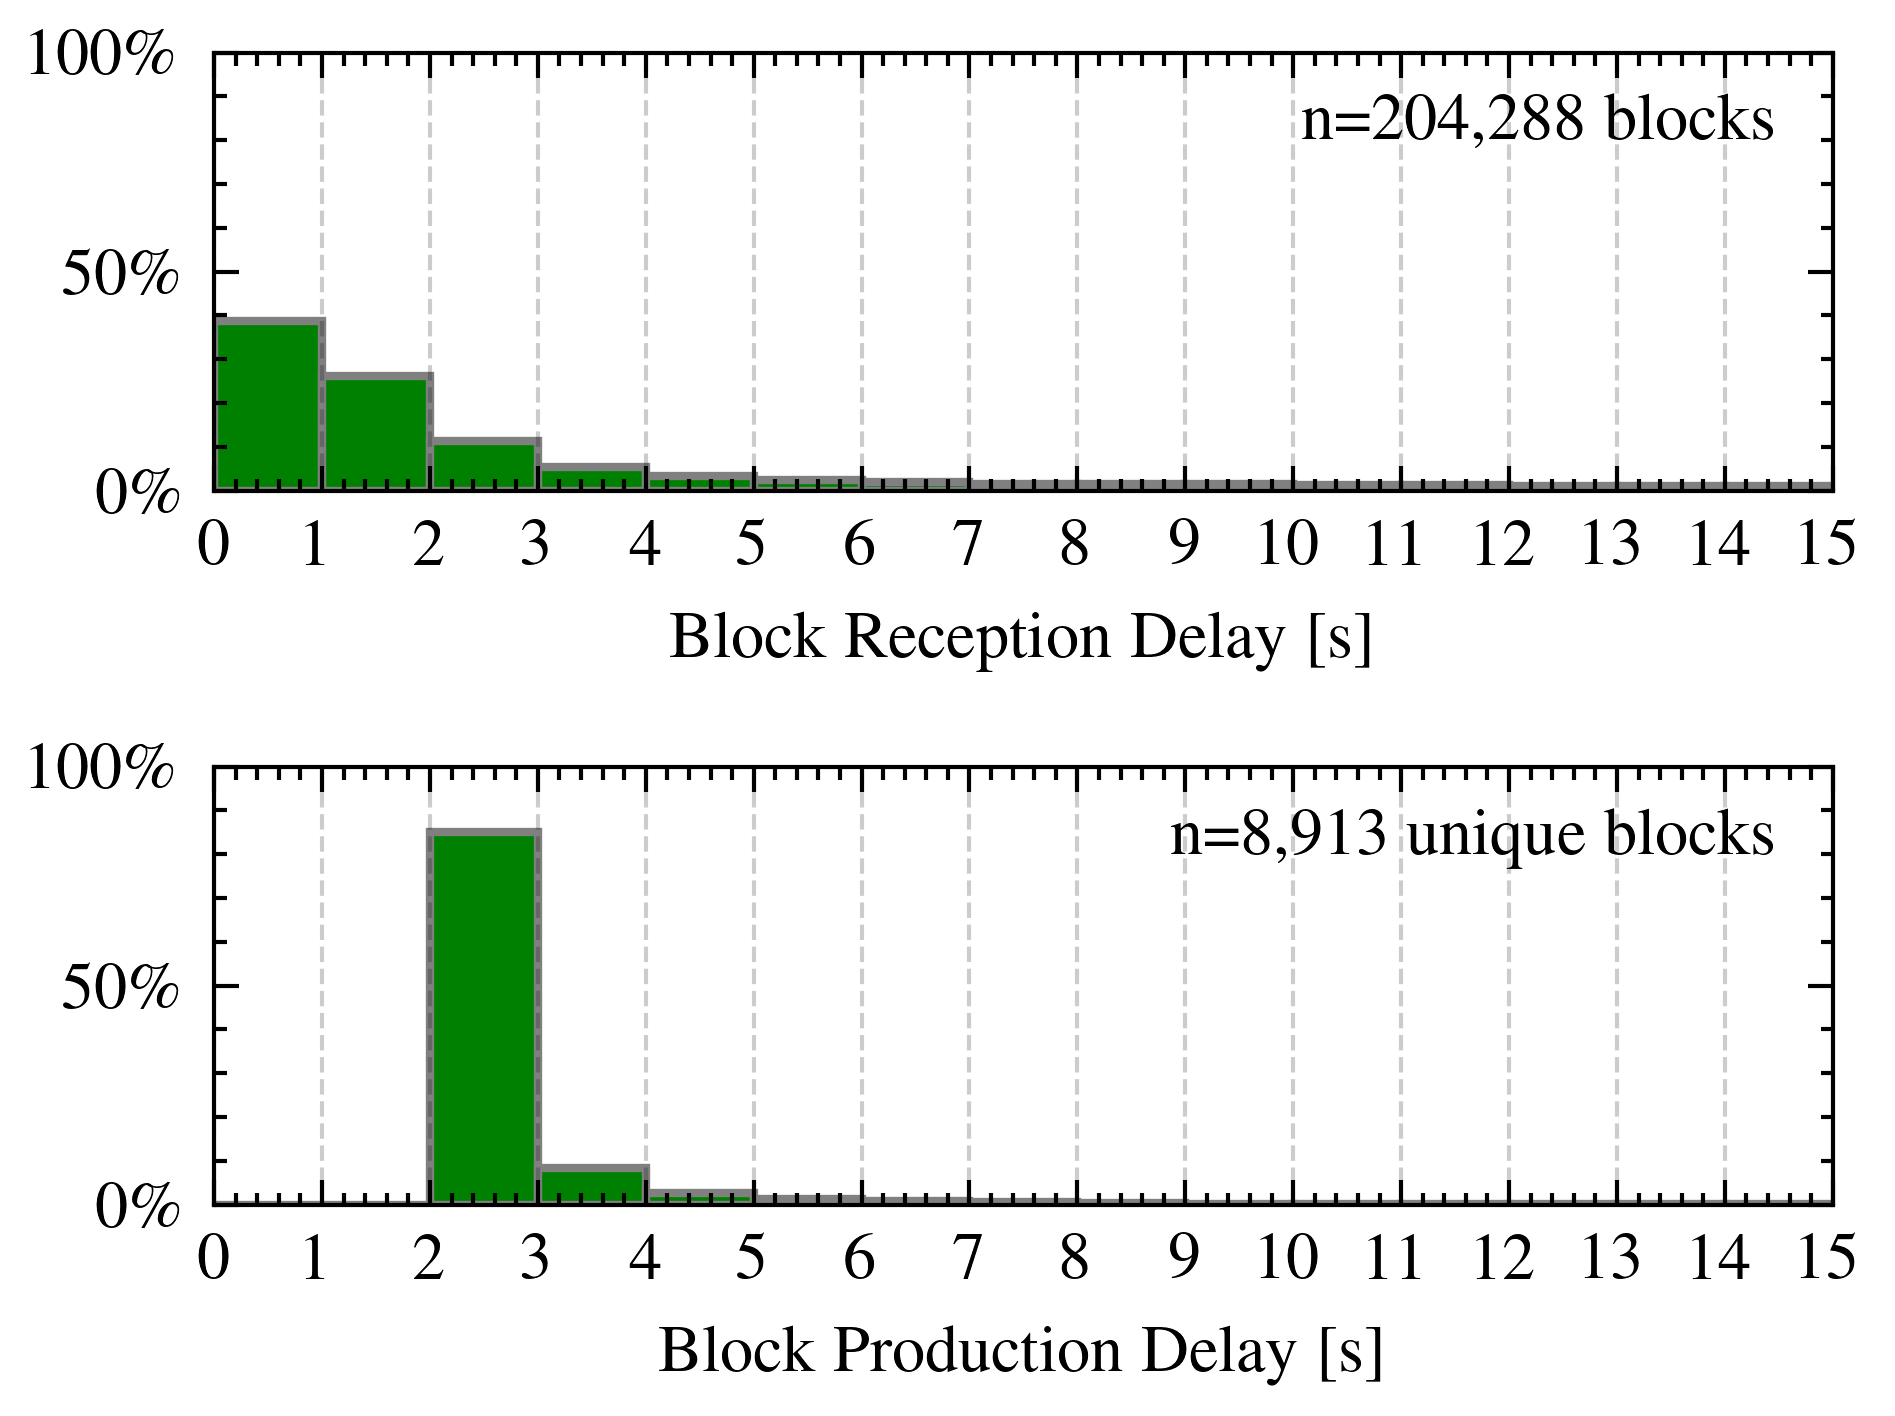
\includegraphics{multi/time_elapsed_both.png}
  \caption{Top: The time it took for every robot to receive each new block of information. In our experiments, 60\% of the blocks were consistently received in under $2$~seconds, which justifies the choice for a block period $T_{block}=2$s. Bottom: The time it took for a new block to be produced. With $T_{block}=2$s, the minimum and ideal production delay is $2$~seconds. An additional delay is introduced due to network delays (temporary unavailability of the preferred block producer, for instance). In our experiments, 90\% of the blocks were produced within $2$ to $3$~seconds, which means that the blockchain is working under nominal conditions throughout all experiments. Note: these plots are generated from the combined data of all experiments performed in this study}
  \label{fig:block-histograms}
\end{figure}

\subsubsection{Data storage costs}

In previous research~\cite{pacheco_ants_2020,StrCasDor2018:aamas}, the block period was $15$~seconds. With a block period of $2$~seconds, we expect that the costs of storing the blockchain will be higher since the amount of data stored depends on the number of blocks created, and also on number of transactions executed by the robots. 

Figure~\ref{fig:data-storage} shows the size (in MB) of the folder where the blockchain is stored. The data storage required increases linearly over the course of the experiment, and sublinearly with the number of robots in the swarm. At the end of the experiment, the occupied card storage is about $8$~MB (i.e., our experiment carried out on a $16$~GB SD could be performed $2000$~times before running out of storage space). Furthermore, the robots do not need to store the complete history of the blockchain, as it contains information which is no longer relevant for their operation. \cite{nishida_suppressing_2018} presents an approach to reducing the blockchain storage costs in robot swarms. The role of storing the complete blockchain can be distributed between robots, or externally sourced as connectivity becomes available, while the robots may leverage cryptography to check for database consistency.

In light of this, we do not expect memory to pose an scalability problem in a real deployment because: 1)~the cost is reasonable given current data storage technology; and 2)~blockchain cryptography can be leveraged to reduce the storage costs in robot swarms.

<<<<<<< HEAD
=======
\begin{figure}
    \begin{minipage}[c]{0.5\textwidth}
        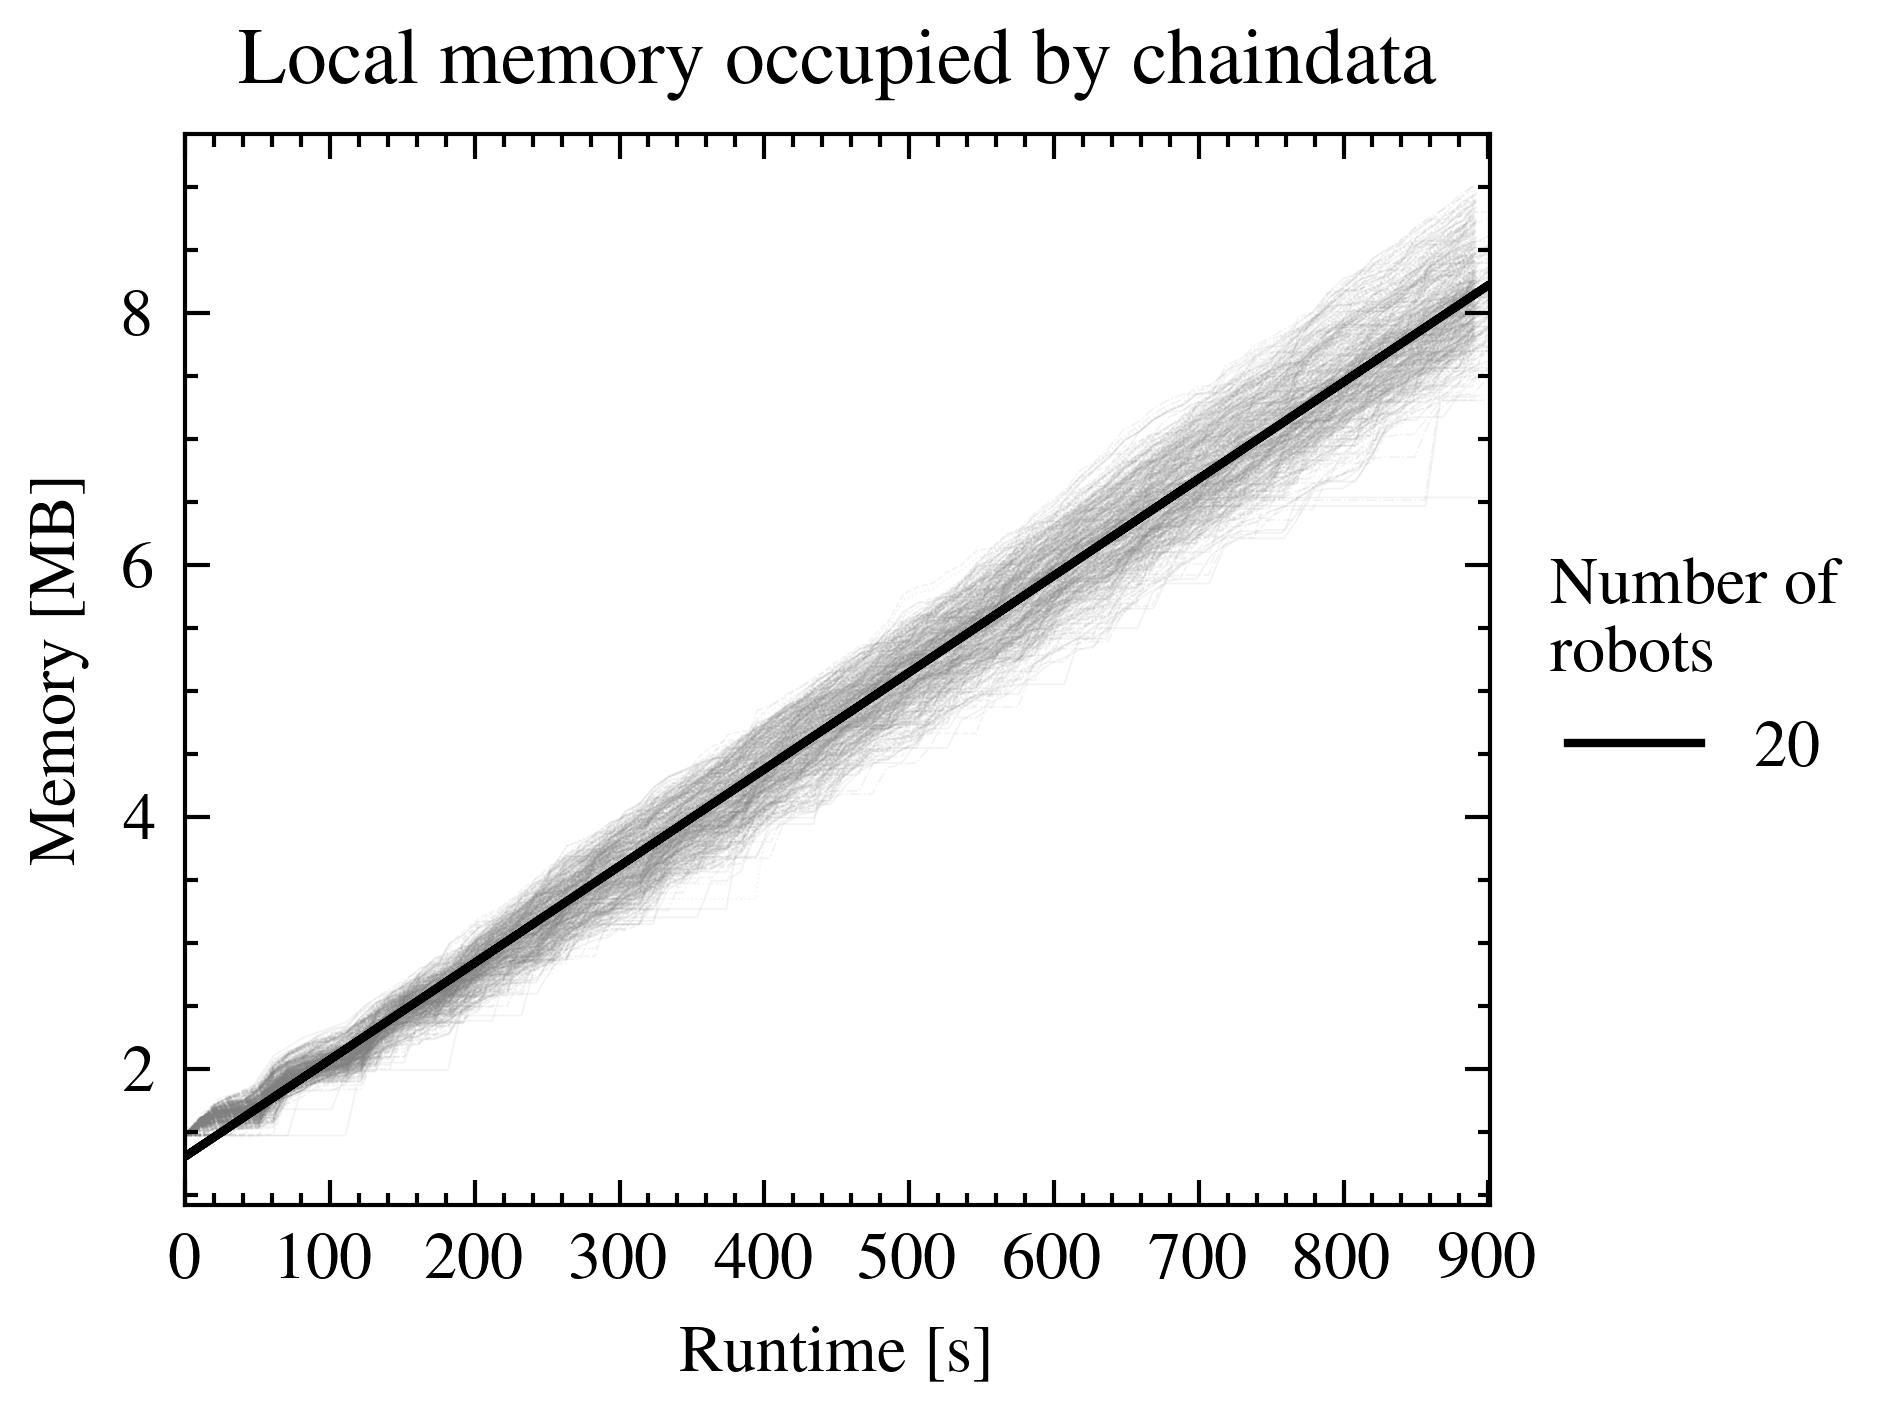
\includegraphics{multi/local_memory.png}
    \end{minipage}\hfill
    \begin{minipage}[c]{0.48\textwidth}
        \caption{The storage space occupied by the blockchain grows linearly over time. The lines in gray are the exact values over time; while the colored lines are linear regressions for three different swarm sizes over $20$~repetitions} 
        \label{fig:data-storage}
    \end{minipage}
\end{figure}
>>>>>>> 49cc2080c4286f2f49bc3ad41a886fb75c97fb85


% \begin{figure}
%   \centering
%   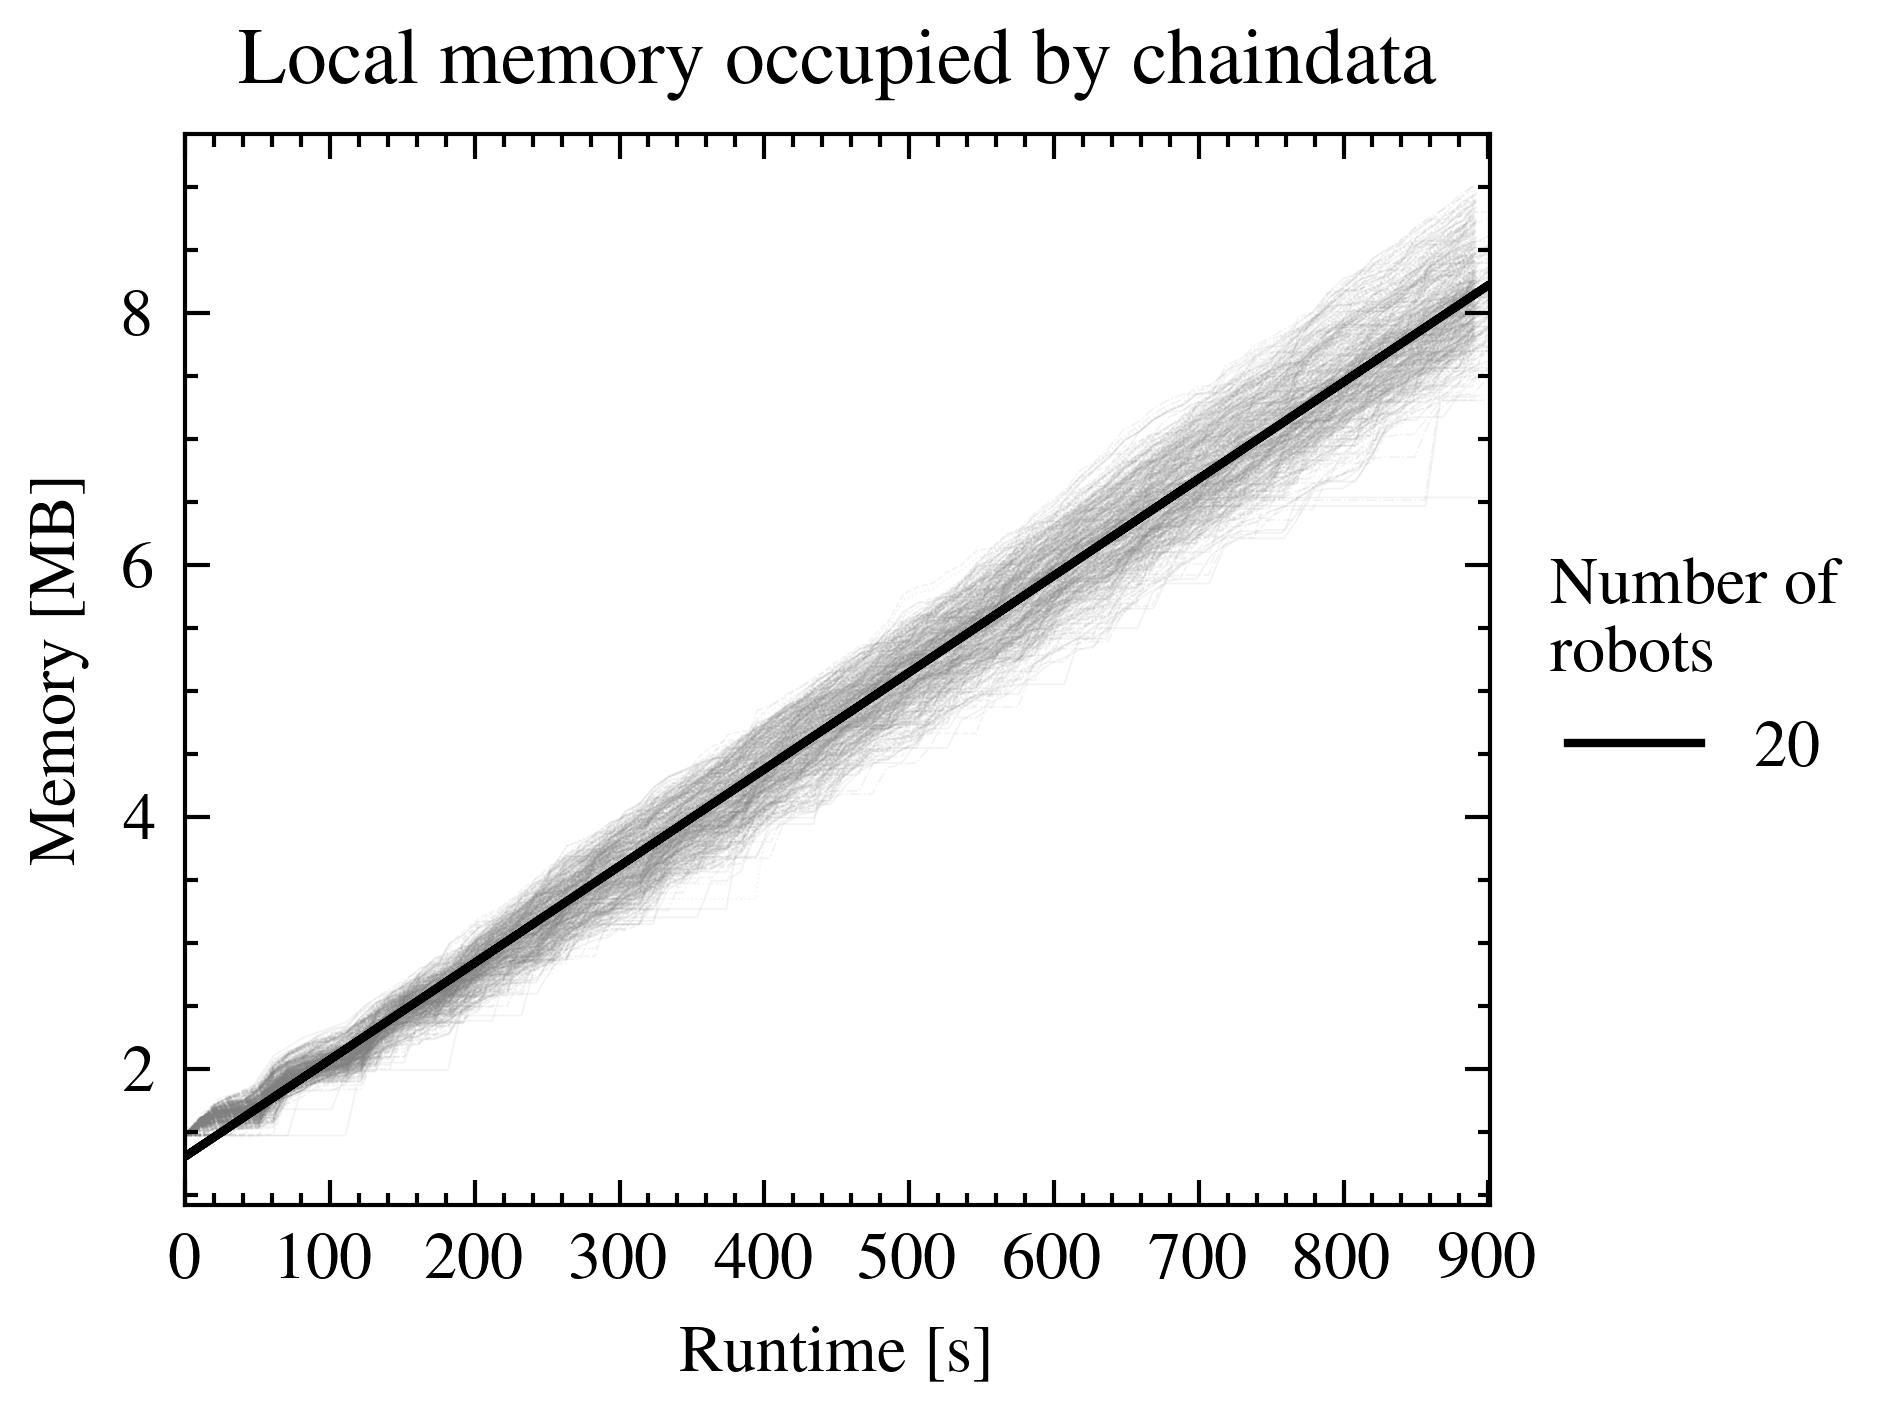
\includegraphics{multi/local_memory.png}
%   \caption{The storage space occupied by the blockchain grows linearly over time. The lines in gray are the exact values over time; while the colored lines are linear regressions for three different swarm sizes over $20$~repetitions} 
%   \label{fig:data-storage}
% \end{figure}


%To analyze the impact on performance of the delay introduced by the blockchain on the swarm, we apply the same controller -- individualist controller.
%\begin{figure}
%  \centering
%  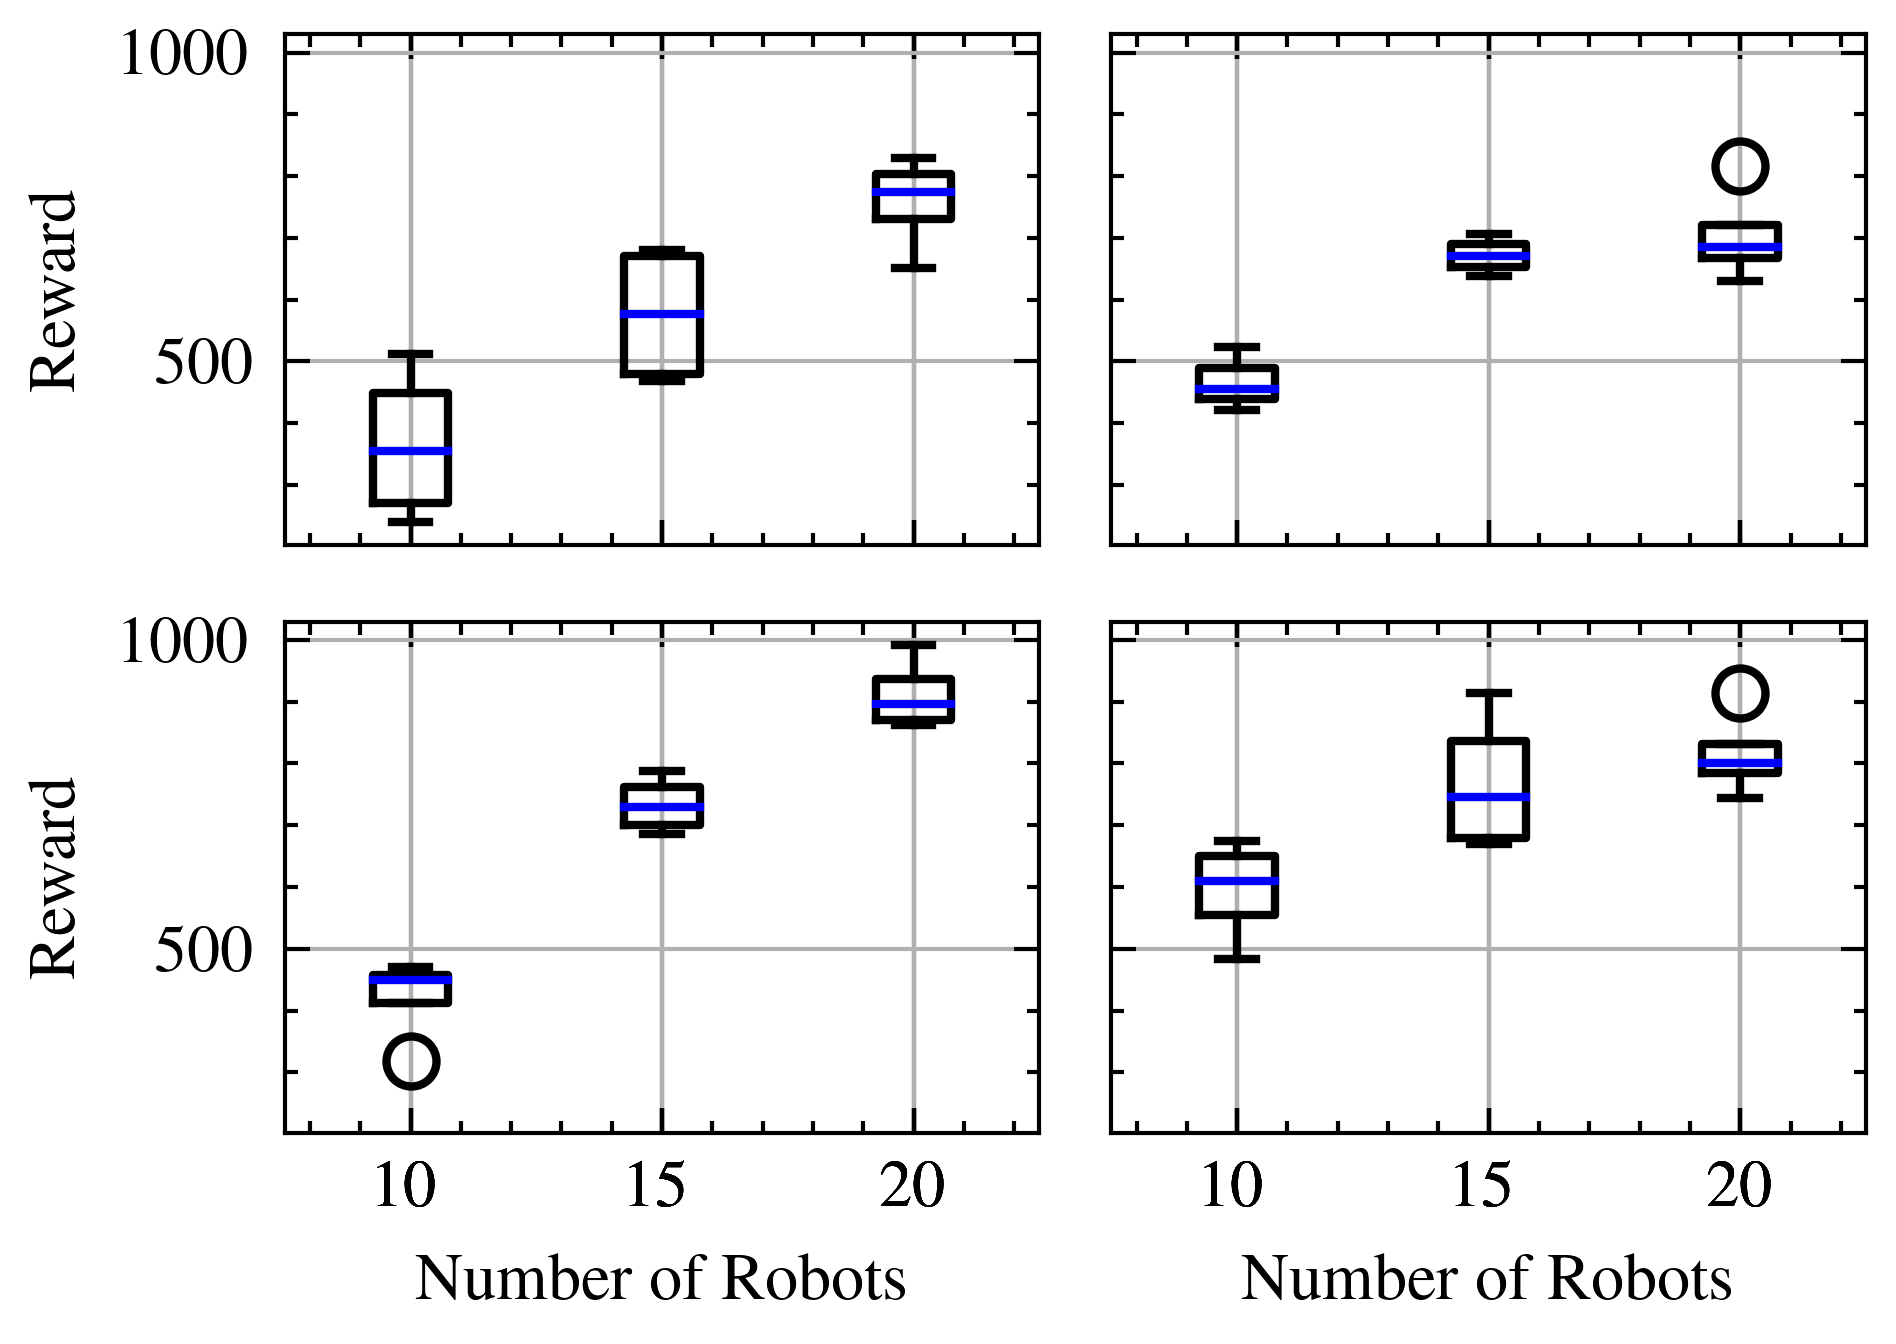
\includegraphics{test116/value_bp_Robots.png}
%  \caption{} 
%  \label{fig:experiment3}
%\end{figure}
%\begin{figure}
%  \centering
%  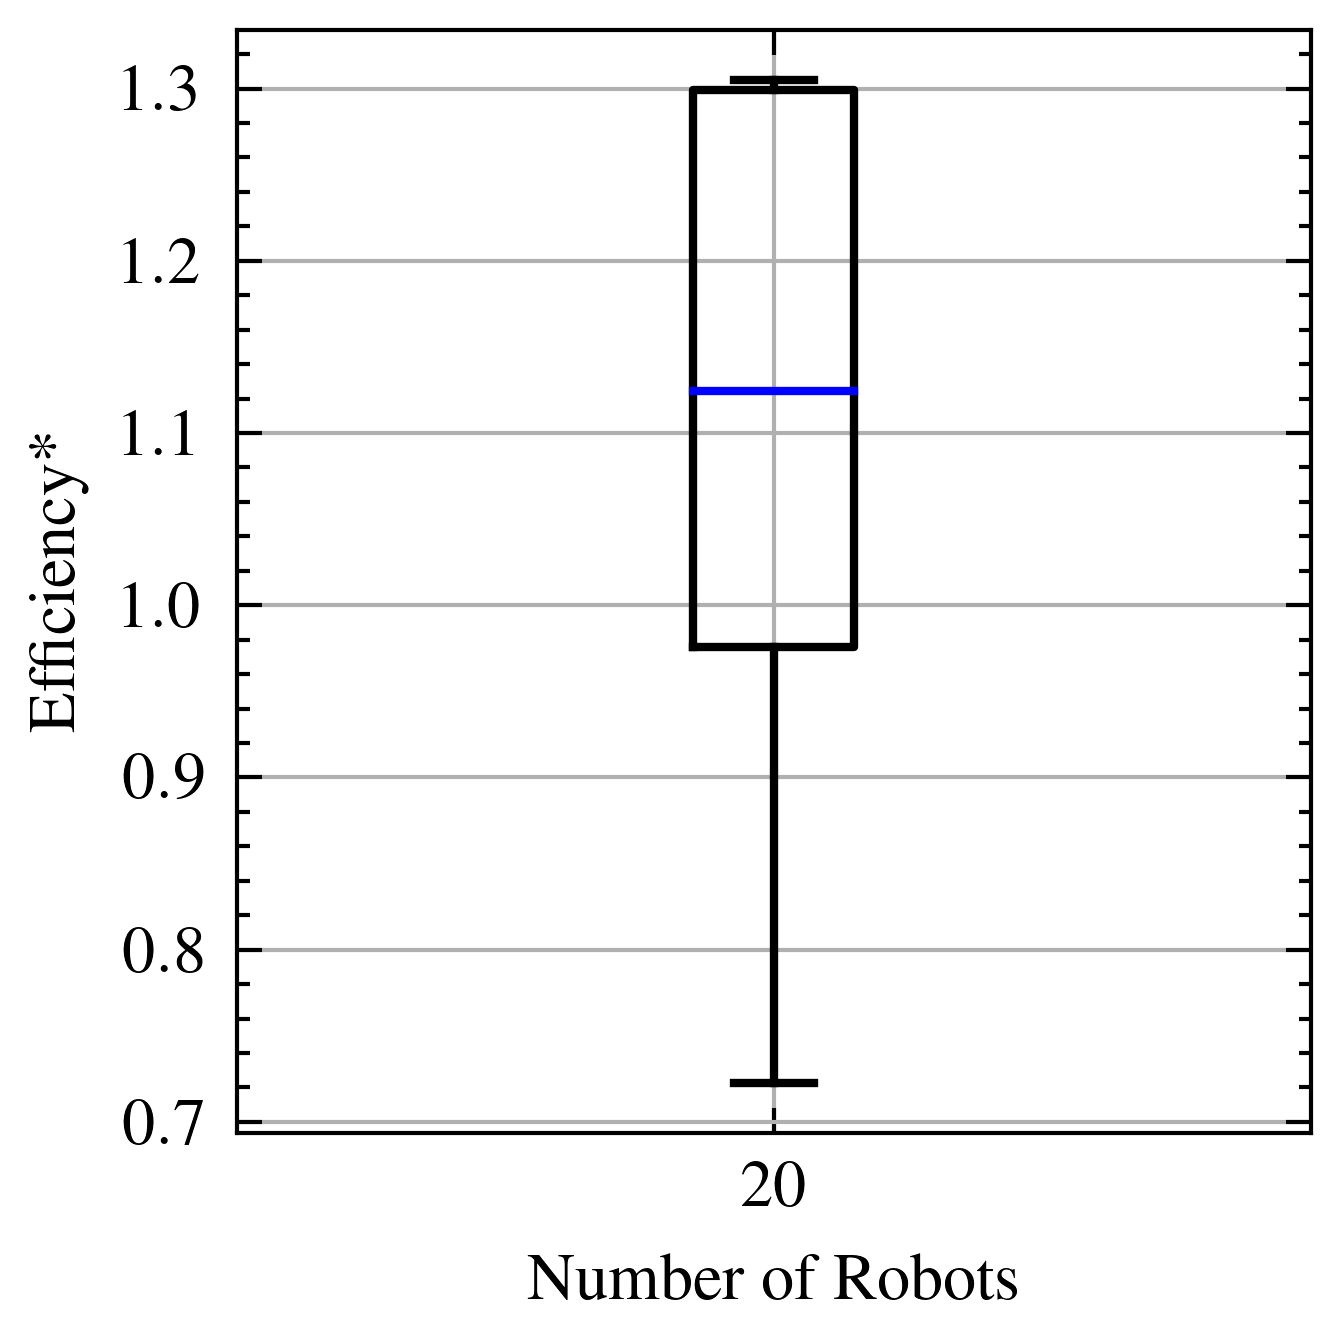
\includegraphics{test116/efficiency_bp_Robots.png}
%  \caption{} 
%  \label{fig:experiment3}
%\end{figure}

\subsubsection{Performance}



\begin{figure}
\centering
\begin{minipage}{.495\textwidth}
  \centering
  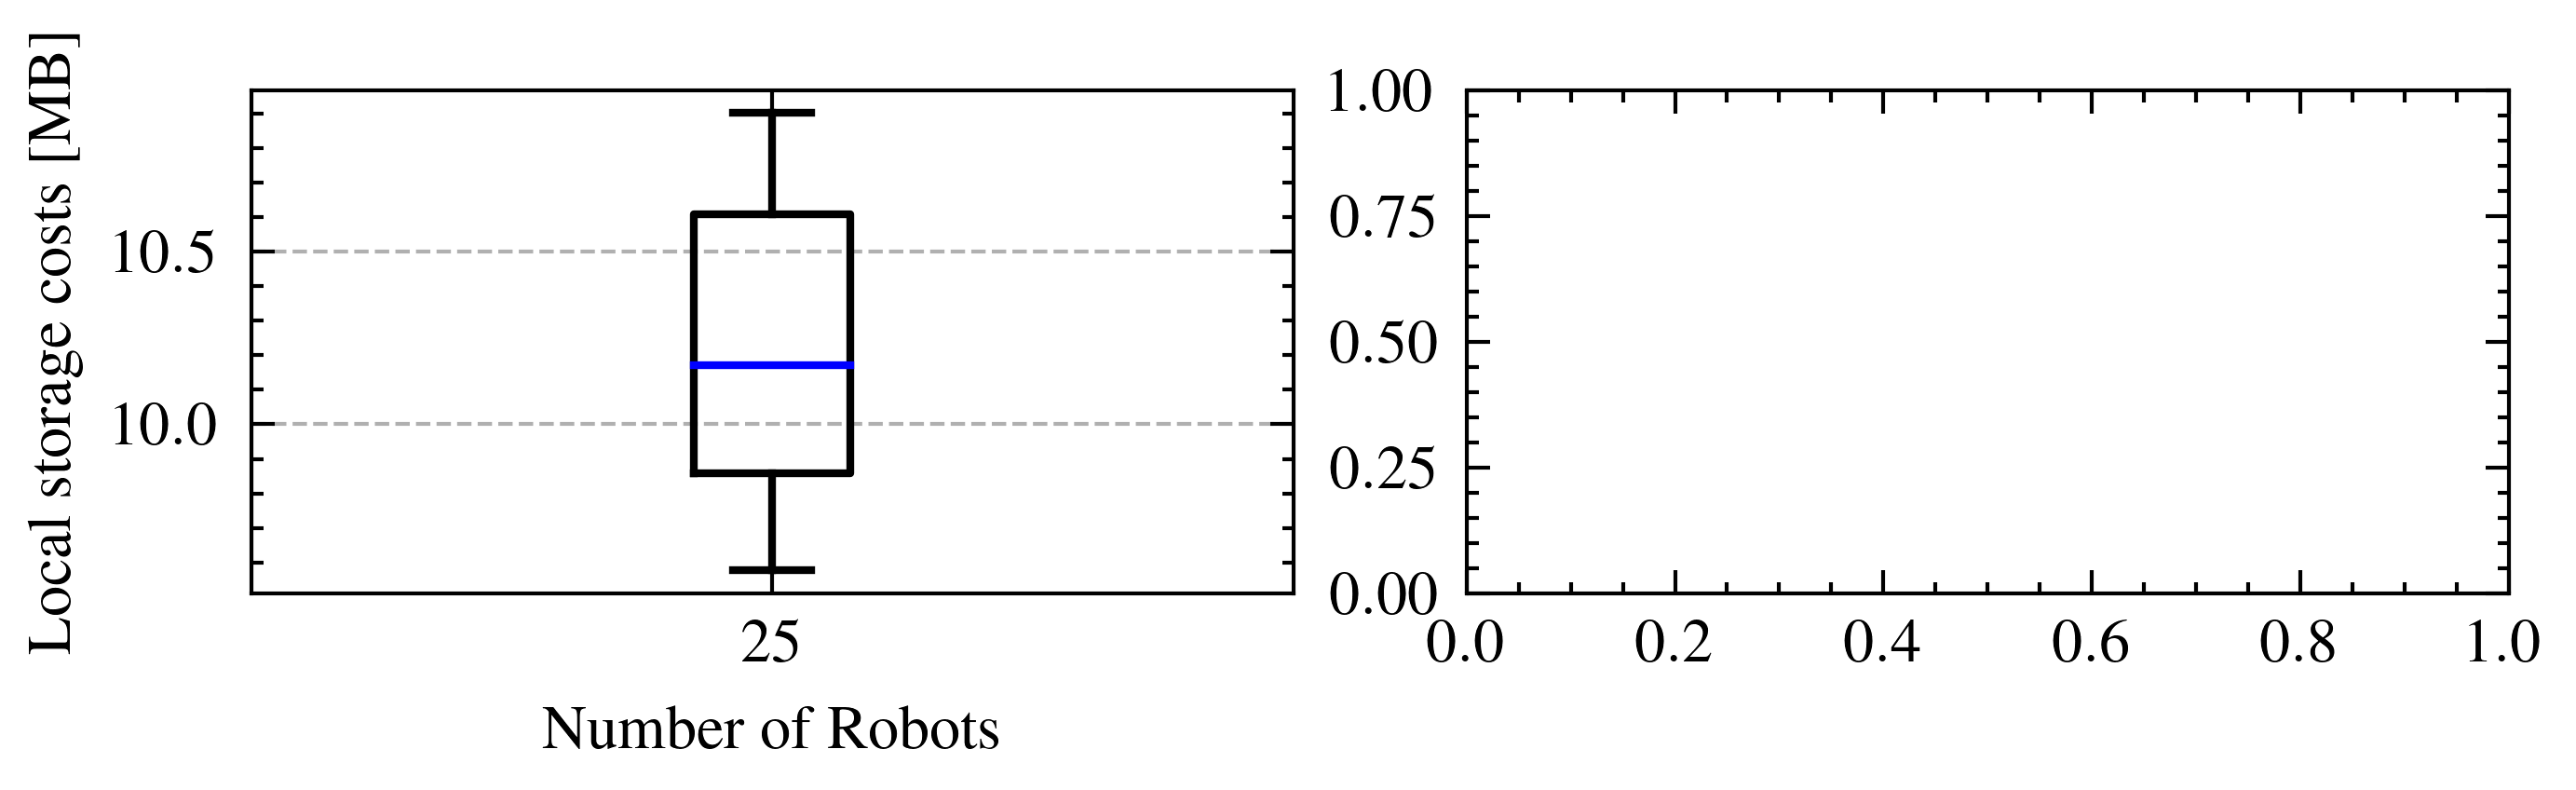
\includegraphics{test120_scaling/storage_bp_Robots_MB.png}
  \label{fig:data-storage}
\end{minipage}
\centering
\begin{minipage}{.495\textwidth}
  \centering
  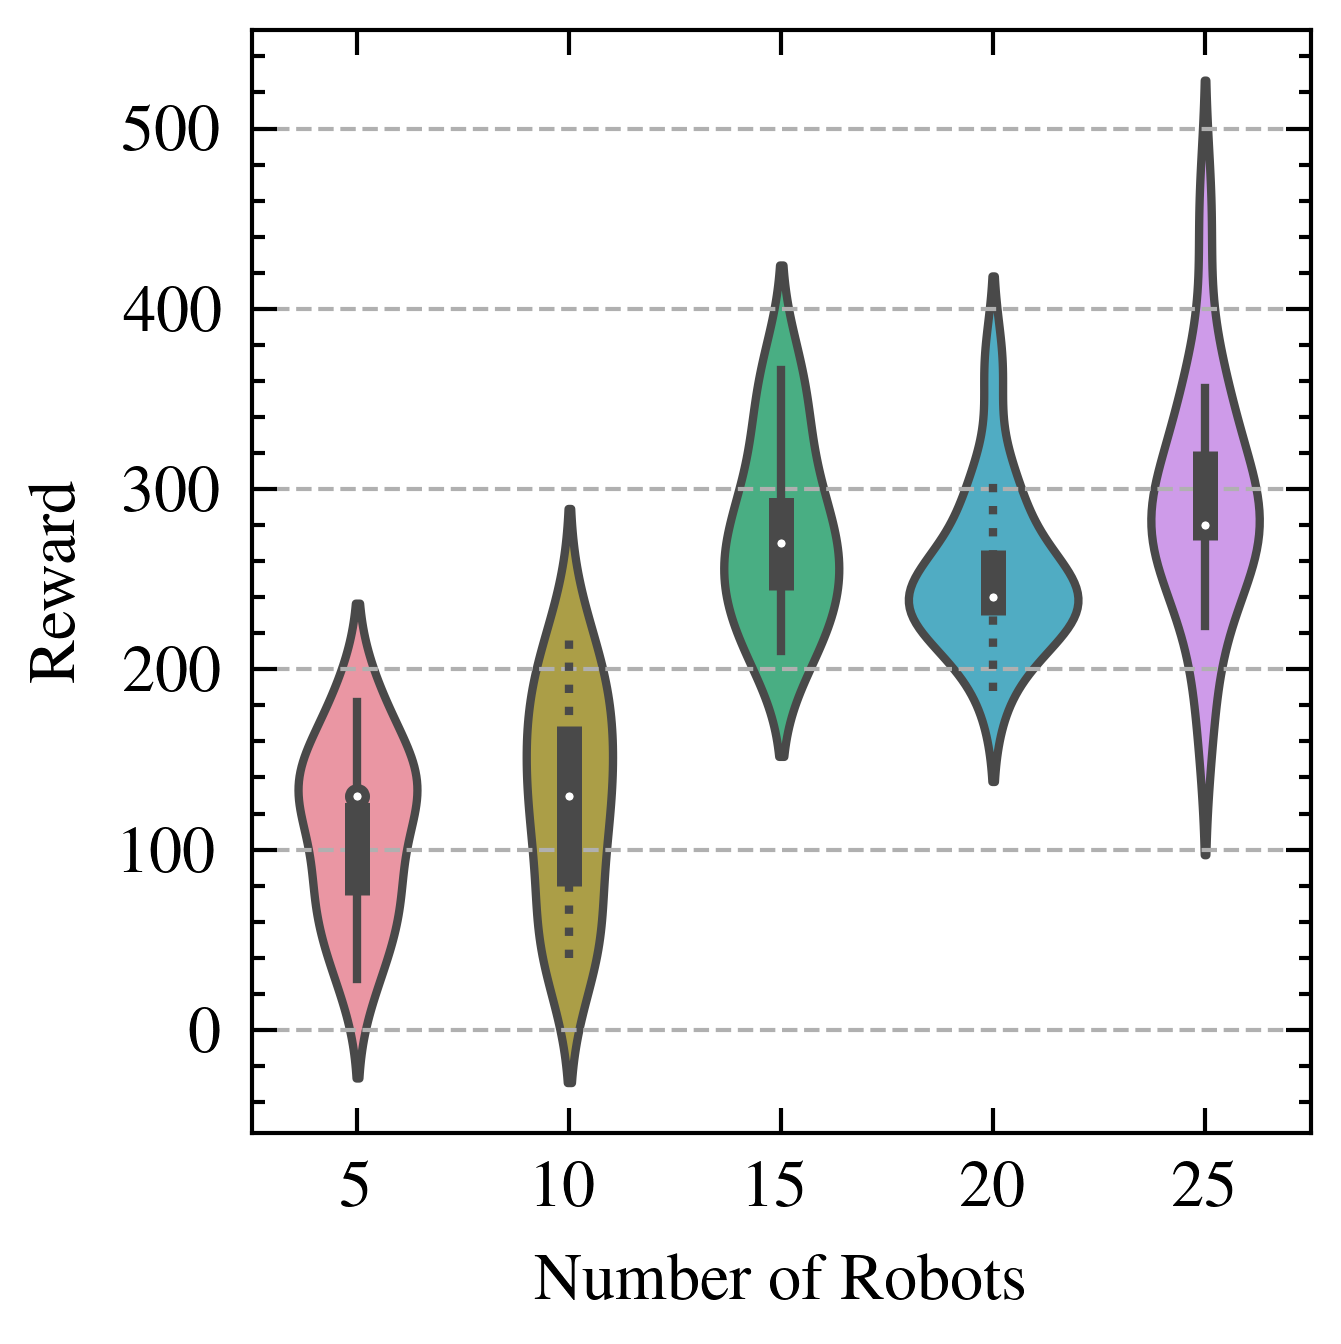
\includegraphics{test120_scaling/performance_bp_Robots_VALUE.png}
  \label{fig:performance}
\end{minipage}
\caption{The storage space occupied by the blockchain grows linearly over time. The lines in gray are the exact values over time; while the colored lines are linear regressions for three different swarm sizes over $20$~repetitions} 
\end{figure}


\subsection{Adaptability}
\label{subsec:adaptability}

\subsubsection{Scattered distribution}
%In the abundant distribution $5$\% of the environment floor area is covered with uniformly distributed patches. Each patch has a diameter of 12~$cm$ and contains $8$~resources. 70\% of the patches are red, while there is 10\% of each green, blue and yellow.

The environment is considered abundant since it is relatively easy for the robots to independently discover resources. In such environments, individualist foragers can perform well enough~\cite{pitonakova_icr_2018,wilson_sociobiology_2000}, or even better if the benefits of cooperation do not overcome the damage from interference. In Figure~\ref{fig:abundant-value} the total reward collected saturates after $2$ recruits per patch, and begins to drop at $5$ recruits. Cooperating robots share the location of higher quality patches, and are thus capable of retrieving more reward with an increased scouting efficiency (Figure~\ref{fig:abundant-eff-exp}). On the other hand, as the number of recruits becomes too high (more than $2$ recruits) interference and lack of robots available for scouting start to harm the performance of the swarm.

\begin{figure}
\centering
\begin{minipage}{.495\textwidth}
  \centering
  \includegraphics{test120/value_bp_Recruits_VALUE.png}
  \caption{A figure}
  \label{fig:scattered-value}
\end{minipage}
\centering
\begin{minipage}{.495\textwidth}
  \centering
  \includegraphics{test120/efficiency_bp_Recruits_SCOUT_DIST.png}
  \caption{Another figure}
  \label{fig:scattered-eff-exp}
\end{minipage}
\end{figure}

%\begin{figure}
% \begin{minipage}{.495\textwidth}
%   \centering
%   \includegraphics{test117/value_bp_Recruits_DIST.png}
%   \caption{A figure}
%   \label{fig:abundant-dist}
% \end{minipage}
% \begin{minipage}{.495\textwidth}
%   \centering
%   \includegraphics{test117/efficiency_bp_Recruits_RECRUIT_DIST.png}
%   \caption{A figure}
%   \label{fig:abundant-eff-for}
% \end{minipage}
% \end{figure}


\subsubsection{Concentrated distribution}
%In the scarce distribution $4$\% of the environment floor area is covered with uniformly distributed patches. Each patch has a diameter of 30~$cm$ and contains $15$~red berries. 

The blockchain coordinated swarm is capable to retrieve $50$\% to $100$\% more reward (Figure~\ref{fig:scarce-value}) and be $2$~-$3$~times more efficient during scouting (Figure~\ref{fig:scarce-eff-scout}). In this environment, it is hard for the scouts to find resources due to relative scarcity, but it is easier for foragers as the patches are quite large and thus inferences do not show a big impact until $5$~recruits per patch. Coordination can be very valuable in such an environment.

\begin{figure}
\centering
\begin{minipage}{.495\textwidth}
  \centering
  \includegraphics{test120_concentrated/value_bp_Recruits_VALUE.png}
  \caption{A figure}
  \label{fig:concentrated-value}
\end{minipage}
\begin{minipage}{.495\textwidth}
  \centering
  \includegraphics{test120_concentrated/efficiency_bp_Recruits_SCOUT_DIST.png}
  \caption{Another figure}
  \label{fig:concentrated-eff-scout}
\end{minipage}
\end{figure}

% \begin{figure}
% \begin{minipage}{.495\textwidth}
%   \centering
%   \includegraphics{test117_scarce_big/value_bp_Recruits_DIST.png}
%   \caption{A figure}
%   \label{fig:scarce-dist}
% \end{minipage}
% \begin{minipage}{.495\textwidth}
%   \centering
%   \includegraphics{test117_scarce_big/efficiency_bp_Recruits_RECRUIT_DIST.png}
%   \caption{A figure}
%   \label{fig:scarce-eff-recruit}
% \end{minipage}
% \end{figure}

\subsubsection{Hotspot distribution}
%In the hotspot distribution $3$\% of the environment floor area is covered with patches following a normal distribution (0.25*1.825, 0.15*1.825) around a center point. Each patch has a diameter of 14~$cm$ and contains $8$~red berries. 

The blockchain coordinated swarm is capable to retrieve more than double the reward (Figure~\ref{fig:hotspot-value}) and be $2$~-$5$~times more efficient during scouting (Figure~\ref{fig:hotspot-eff-exp}). This occurs because the scouting robots which move in the direction of the hotspot are very successful, while others robots do not find any resources. The ability to aggregate and share information prevents unsuccessful robots from idling or wasting energy performing redundant exploration. Conversely, given the tight aggregation of resources, the foraging efficiency quickly drops as the number of recruits increases due higher physical interference between robots. %(Figure~\ref{fig:hotspot-eff-for})

\begin{figure}
\centering
\begin{minipage}{.495\textwidth}
  \centering
  \includegraphics{test120_hotspot/value_bp_Recruits_VALUE.png}
  \caption{}
  \label{fig:hotspot-value}
\end{minipage}
\begin{minipage}{.495\textwidth}
  \centering
  \includegraphics{test120_hotspot/efficiency_bp_Recruits_SCOUT_DIST.png}
  \caption{Another figure}
  \label{fig:hotspot-eff-exp}
\end{minipage}
\end{figure}

%\begin{figure}
% \begin{minipage}{.495\textwidth}
%   \centering
%   \includegraphics{test117_patchy_single/efficiency_bp_Recruits_RECRUIT_DIST.png}
%   \caption{A figure}
%   \label{fig:hotspot-eff-for}
% \end{minipage}
% \begin{minipage}{.495\textwidth}
%   \centering
%   \includegraphics{test117_patchy_single/value_bp_Recruits_DIST.png}
%   \caption{A figure}
%   \label{fig:hotspot-dist}
% \end{minipage}
% \end{figure}


% \subsubsection{Litter distribution}
% \todo{maybe remove litter -- or make it more similar to pitanokovas for comparison (15 per patch is too much for "litter")}
% %In the litter distribution $2$\% of the environment floor area is covered with uniformly distributed patches. Each patch has a diameter of 10~$cm$ and contains $15$~red berries.
%  The improvement is about $50$\% in the total reward collected, and the scouting efficiency doubles for $3$ or more recruits. Due to the small size of resources, the system very prone to damage from interference as the foraging efficiency drops significantly as the number of recruits increases (Figure~\ref{fig:scarce-eff-recruit}). Generally speaking, collaborating swarms in small, sparse and low quality patches have been shown to not fare well due to the reinforced effect of informational and physical interference [pit]. Despite this, the blockchain coordinated swarm shows an improved performance, although not as drastic as in the other environments.

% \begin{figure}
% \centering
% \begin{minipage}{.495\textwidth}
%   \centering
%   \includegraphics{test117_litter/value_bp_Recruits_VALUE.png}
%   \caption{A figure}
%   \label{fig:litter-value}
% \end{minipage}
% \begin{minipage}{.495\textwidth}
%   \centering
%   \includegraphics{test117_litter/value_bp_Recruits_DIST.png}
%   \caption{A figure}
%   \label{fig:litter-dist}
% \end{minipage}
% \end{figure}

% \begin{figure}
% \centering
% \begin{minipage}{.495\textwidth}
%   \centering
%   \includegraphics{test117_litter/efficiency_bp_Recruits_SCOUT_DIST.png}
%   \caption{Another figure}
%   \label{fig:litter-eff-scout}
% \end{minipage}
% \begin{minipage}{.495\textwidth}
%   \centering
%   \includegraphics{test117_litter/efficiency_bp_Recruits_RECRUIT_DIST.png}
%   \caption{A figure}
%   \label{fig:litter-eff-rec}
% \end{minipage}
% \end{figure}

\section{Conclusions and Future Work}
\label{sec:conclusion}

We showed that very simple rules contained in a decentralized smart contract coordinator can indeed be used to improve the performance of a robot swarm, while keeping reasonable data storage costs and manageable delay in the control loop. The study is limited in the sense that we do not fully explore the coordination potential of smart contracts: we use a static smart contract, which does not adapt its rules according to the quantity of patches that are present in the environment, nor according to the properties (quality, distance or quantity) of the resources they contain.

In future work, we will extend the ability of the smart contract to introduce coordination rules which are not feasible in robot swarm systems that do not exploit a shared knowledge database. Optimal foraging theory, for instance, dictates that resources below a quality threshold should be ignored in order to improve the energetic balance of the swarm. 

%The number of recruits per patch should also be regulated according to the properties of that patch (i.e., larger patches with more resources and better quality should have more recruits allocated to them).



\bibliographystyle{splncs04}
\bibliography{mybibliography}
\end{document}
